\documentclass{article}

\setlength{\emergencystretch}{15pt}

\usepackage{graphicx}

\usepackage{amsmath}

\begin{document}
\section{Herleitung}
\subsection{Methode}
Wenn der Korrekturterm 
\begin{equation*}
    y=-\frac{p(x)}{\prod_{j=1;j\neq k}^{n}(x-z_j^{(i)})}
\end{equation*}
, mit $z_j^{(i)} = z_j$ für $j=1;2;\dots;n$, umgestellt wird
\begin{align*}
    y&=-\frac{p(x)}{\prod_{j=1;j\neq k}^{n}(x-z_j)} \\
     &=-\frac{\prod_{j=1}^{n}(x-z_j)}{\prod_{j=1;j\neq k}^{n}(x-z_j)} \\
     &=-(x-z_k)
\end{align*}
kann erkannt werden, dass es sich um eine lineare Funktion mit der Nullstelle $z_k$ handelt. Bei der Weierstraß-Iteration wird der Wert $z_k^{(i)}$ mit dem Korrekturterm mit $x=z_k^{(i)}$ addiert. Das kann vereinfacht werden:
\begin{align*}
    z_k^{(i+1)}&=z_k^{(i)}-(z_k^{(i)}-z_k) \\
    &= z_k \\
\end{align*}
Daraus folgt, dass, wenn alle anderen Nullstellen gefunden wurden, die Weierstraß-Iteration konvergiert. \\
\\
Wenn jetzt allerdings noch nicht alle anderen Nullstellen gefunden wurden ergibt der Korrekturterm eine gebrochen rationale Funktion. Diese Verhält sich ähnlich wie die zuvor beschriebene lineare Funktion. Es bilden sich jedoch Definitionslücken des Korrekturterms an den Werten der linearen Faktoren. Außerdem weicht die Funktion teilweise von der zuvor beschriebenen linearen Funktion ab. Diese Abweichung wird allerdings mit zunehmender Distanz von den undifinierten Stellen geringer, da der gebrochene Term immer kleiner wird. \\
\\
Um die Nullstelle $z_k$ findet in jedem Fall ein Vorzeichenwechsel von plus zu minus statt. Das bedeutet dass vor der Nullstelle sich nur positive Werte befinden und nach der Nullstelle nur negative.
Dabei sind die seltenen Fälle, dass in der Nähe eine Definitionslücke befindet, außgenommen. Darauf wird später eingegangen.
Das bedeutet für die Weierstraß-Iteration, dass sich der Wert an die Nullstelle annährt, da mit einer annährung an die Nullstelle immer kleinere Schritte gegangen wird.\\
Das bedeutet letzendlich dass die Weierstraß-Iteration für jede Nullstelle konvergiert. Allerdings gibt es Definitionslücken. \\
\begin{figure}[h]
    \centering
    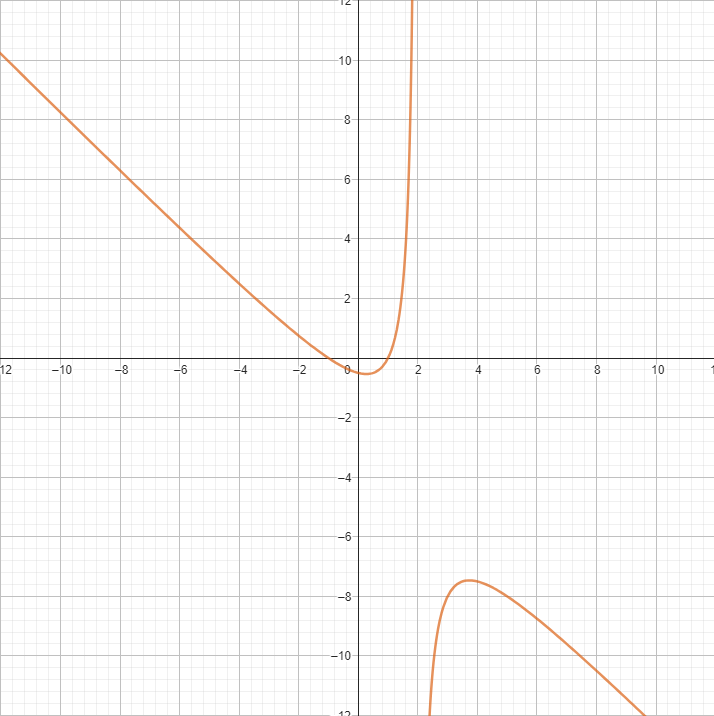
\includegraphics[scale=.4]{(x^2-1)geteilt(x-2).png} \\
    \vspace*{0.3cm}
    Graph der Funktion $\frac{x^2-1}{x-2}$\\
    Mit GeoGebra CAS erstellt\footnote{}
\end{figure} \\
Um diese steigt oder fällt die Funktion rasant. Wenn sich $z_k^{(i)}$ in diesem Bereich befindet kann eine verfälschte Korrektur herrauskommen. Das führt zu mehr Iterationsschritten, ist allerdings sehr selten. Außerdem kann es vorkommen, dass sich $z_k^{(i)}$ auf einer undifinierten Stelle befindet. Das führt zu einem Fehler bei der Iteration, ist aber, wenn unterschiedliche Werte als Startpunkte genommen werden, extrem unwahrscheinlich. Zuletzt kann es vorkommen, dass sich Nullstellen so nahe aneinander befinden, dass eine Nullstelle in dem Ereignisbereich\footnote{Der Ereignisbereich ist in diesem Fall der Bereich in dem der gebrochene Term, um eine Definitionslücke, einen größeren Einfluss als der Rest hat. Der Ereignisbereich beginnt und endet mit den Extremstellen um die Definitionslücke.} einer Definitionslücke steht und nicht erreicht werden kann. Das führt dazu dass die Weierstraß-Iteration erst nach unendlich Iterationen, da erst nach unendlich Iterationen die anderen Nullstellen konvergieren und Definitionslücken wegfallen, die Nullstelle vernünftig nah approximiert, was praktisch nicht möglich ist.

\end{document}